\documentclass[10pt,landscape]{article}
\usepackage{multicol}
\usepackage{graphicx}
\usepackage{calc}
\usepackage{ifthen}
\usepackage{color}
\usepackage[landscape]{geometry}

\ifthenelse{\lengthtest { \paperwidth = 11in}}
	{ \geometry{top=.05in,left=.05in,right=.05in,bottom=.05in} }
	{\ifthenelse{ \lengthtest{ \paperwidth = 297mm}}
		{\geometry{top=1cm,left=1cm,right=1cm,bottom=1cm} }
		{\geometry{top=1cm,left=1cm,right=1cm,bottom=1cm} }
	}

% Turn off header and footer
\pagestyle{empty}
 

% Redefine section commands to use less space
\makeatletter
\renewcommand{\section}{\@startsection{section}{1}{0mm}%
                                {-1ex plus -.5ex minus -.2ex}%
                                {0.5ex plus .2ex}%x
                                {\normalfont\large\bfseries}}
\renewcommand{\subsection}{\@startsection{subsection}{2}{0mm}%
                                {-1explus -.5ex minus -.2ex}%
                                {0.5ex plus .2ex}%
                                {\normalfont\normalsize\bfseries}}
\renewcommand{\subsubsection}{\@startsection{subsubsection}{3}{0mm}%
                                {-1ex plus -.5ex minus -.2ex}%
                                {1ex plus .2ex}%
                                {\normalfont\small\bfseries}}
\makeatother

% Define BibTeX command
\def\BibTeX{{\rm B\kern-.05em{\sc i\kern-.025em b}\kern-.08em
    T\kern-.1667em\lower.7ex\hbox{E}\kern-.125emX}}

% Don't print section numbers
\setcounter{secnumdepth}{0}


\setlength{\parindent}{0pt}
\setlength{\parskip}{0pt plus 0.5ex}


% -----------------------------------------------------------------------

\begin{document}

\raggedright
\footnotesize
\begin{multicols}{3}


% multicol parameters
% These lengths are set only within the two main columns
%\setlength{\columnseprule}{0.25pt}
\setlength{\premulticols}{1pt}
\setlength{\postmulticols}{1pt}
\setlength{\multicolsep}{1pt}
\setlength{\columnsep}{2pt}

\begin{center}
   
\includegraphics[width=15px]{emer.png}\huge{\textbf{mergent keyboard reference}} \\
   
\end{center}
\section{Global project}
\begin{tabular}{@{}ll@{}}
\verb!Ctrl+S!    & Save project. \\
\verb!Ctrl+left! & Backwards in navigation history \\
\verb!Ctrl+right! & Forwards in navigation history \\
\verb!F5!  & Refresh GUI. \\
\verb!Tab! & Forward through interface \\
\verb!Shift+Tab! & Backwards through interface \\
\verb!Alt+J! & Move global focus left \\
\verb!Ctrl+J! & Move global focus left \\
\verb!Alt+L! & Move global focus right \\
\verb!Ctrl+L! & Move global focus right \\
\end{tabular}

\section{Help Browser}
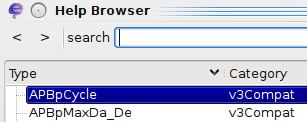
\includegraphics[width=153.5px]{helpbrowser.png} \\
\begin{tabular}{@{}ll@{}}
\verb!F1!  & Help Browser. \\
\verb!Ctrl+S!  & Toggle Search/Find focus. \\
\verb!Tab!  & Switch to search list focus. \\
\verb!Ctrl+n!  & Next element. \\
\verb!Ctrl+p!  & Next element. \\
\verb!Page Up!  & Page Up list or web page. \\
\verb!Page Down!  & Page Down list or web page. \\
\end{tabular}

\section{Tree browser and program code}
\newlength{\MyLen}
\settowidth{\MyLen}{\texttt{letterpaper}/\texttt{a4paper} \ }
\begin{tabular}{@{}ll@{}}
\verb!Any 1-3 chars!    & Find as you type \\
\verb!Alt+F!  & Find from selected node. \\
\verb!Ctrl+I!    & New item below cursor. \\
\verb!Ctrl+F!  & Expand this node. \\
\verb!Shift++!  & Expand this node. \\
\verb!Ctrl+B!  & Collapse this node. \\
\verb!Ctrl+-!  & Collapse this node. \\
\verb!Ctrl+spacebar!  & Selection mode. \\
\verb!Ctrl+P!  & (select) Previous element. \\
\verb!Ctrl+N!  & (select) Next element. \\
\verb!Ctrl+D!  & Delete selected item(s). \\
\verb!Delete!  & Delete selected item(s). \\
\verb!Ctrl+C!  & Copy selected element(s). \\
\verb!Alt+W!  & Copy selected element(s). \\
\verb!Ctrl+X!  & Cut selected element(s). \\
\verb!Ctrl+W!  & Cut selected element(s). \\
\verb!Ctrl+V!  & Paste element(s). \\
\verb!Ctrl+Y!  & Paste element(s). \\
\verb!Ctrl+M!  & Duplicate element(s). \\
\verb!Ctrl+U!  & Page up. \\
\verb!Ctrl+G!  & Deselect. \\
\end{tabular}

\section{css console and text fields}
\begin{tabular}{@{}ll@{}}
\verb!Ctrl+A!    & Beginning of line. \\
\verb!Ctrl+E! & End of line. \\
\verb!Ctrl+K! & Kill text until end of line. \\
\verb!Ctrl+B!  & Move cursor back one character. \\
\verb!Ctrl+F! & Move cursor forward one character. \\
\verb!Ctrl+right! & Move cursor one word forward. \\
\verb!Ctrl+left! & Move cursor one word backwards. \\
\verb!Ctrl+shift+right! & Highlight one word forward. \\
\verb!Ctrl+shift+left! & Highlight one word backwards. \\
\verb!Ctrl+X! & Cut. \\
\verb!Ctrl+C! & Copy. \\
\verb!Ctrl+V! & Paste.
\end{tabular}

\subsection{Text fields}

\includegraphics[width=91px]{path.png} \\
\begin{tabular}{@{}ll@{}}
\verb!Ctrl+L!    & Text completion lookup.  \\
\verb!Ctrl+U!    & Highlight all.
\end{tabular}

\subsection{css console}
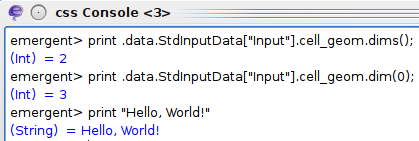
\includegraphics[width=108.5px]{console.png} \\
\begin{tabular}{@{}ll@{}}
\verb!Ctrl+L!    & Clear console buffer history. \\
\verb!Ctrl+L!    & Delete highlighted text. \\
\verb!Ctrl+I!    & Insert tab.
\end{tabular}

\section{DataTables and matrices}
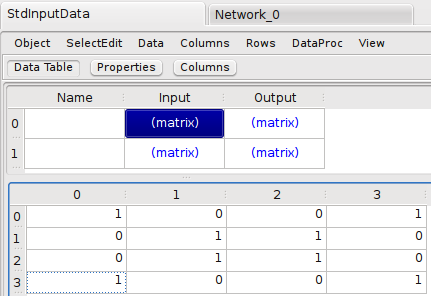
\includegraphics[width=115px]{datatable.png} \\
\begin{tabular}{@{}ll@{}}
\verb!Ctrl+A!    & Beginning of row. \\
\verb!Ctrl+E!    & End of row. \\
\verb!Ctrl+T!    & Switch between table and matrix focus. \\
\verb!Ctrl+F!    & Move one cell right. \\
\verb!Ctrl+B!    & Move one cell left. \\
\verb!Ctrl+P!    & Move one cell up. \\
\verb!Ctrl+N!    & Move one cell down. \\
\verb!Ctrl+C!    & Copy table/matrix cell. \\
\verb!Ctrl+V!    & paste table/matrix cell. \\
\verb!Ctrl+spacebar!    & Start editing cell.
\end{tabular}

\section{New elements in left tree browser}
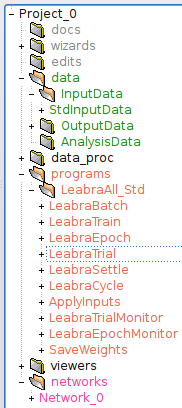
\includegraphics[width=66px]{treebrowser.png} \\
\begin{tabular}{@{}ll@{}}
\verb!do Ctrl+I!    & New Doc \\
\verb!da Ctrl+I!    & New DataTable \\
\verb!la Ctrl+I!    & New Layer \\
\verb!P Ctrl+I!    & New Project \\
\verb!pr Ctrl+I!    & New Program \\
\verb!n Ctrl+I!    & New Network \\
\verb!sp Ctrl+I!    & New Spec
\end{tabular}

\section{New elements in program code}
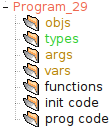
\includegraphics[width=56px]{programcode.png} \\
These sequences insert new items. Press Ctrl+left,left afterwards to navigate back to where you were. \\
\begin{tabular}{@{}ll@{}}
\verb!obj Ctrl+I Type!    & New obj of Type \\
\verb!var Ctrl+I!    & New var \\
\verb!arg Ctrl+I!    & New arg \\
\verb!fun Ctrl+I!    & New fun \\
\verb!init Ctrl+I Name!    & New init code Name \\
\verb!prog Ctrl+I Name!    & New prog code Name \\
\end{tabular}

\section{Middle panel edit dialogs}
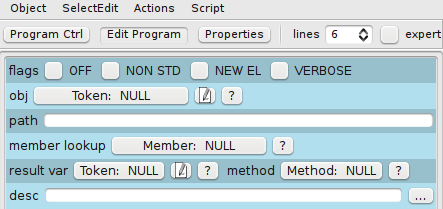
\includegraphics[width=225px]{middlepanel.png} \\
\settowidth{\MyLen}{\texttt{multicol} }
\begin{tabular}{@{}ll@{}} \\
\verb!Tab!    & Next element. \\
\verb!Ctrl+n!    & Next element. \\
\verb!Shift+tab!    & previous element. \\
\verb!Ctrl+p!    & Next element. \\
\verb!Up!    & (numeric field) Increase value. \\
\verb!Down!    & (numeric field) Decrease value. \\
\verb!Up!    & (dropdown) Move up. \\
\verb!Down!    & (dropdown) Move down. \\
\verb!ESC!    & Revert changes. \\
\verb!Ctrl+Enter!    & Apply changes. \\
\verb!Spacebar!    & (buttons) Open token chooser. \\
\verb!Spacebar!    & (flags) Check/uncheck flag. \\
\verb!Ctrl+L!    & (expression fields) Lookup information. \\
\end{tabular}

\section{Program code elements}
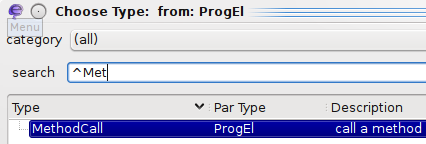
\includegraphics[width=137px]{progel.png} \\
Press Ctrl+i seq Enter, where seq is the shortest subset of the full name needed to put that program element at the top of the list.

\end{multicols}
\end{document}
